\documentclass{beamer}
%\usepackage[utf8]{inputenc}
\usepackage{hyperref}
\usepackage{multicol}
\usepackage{multirow}
\usepackage{hyperref}
\usepackage{graphicx}
\usepackage{booktabs}
\usepackage[font={small,it},labelfont=bf]{caption}

\DeclareMathAlphabet{\mathpzc}{OT1}{pzc}{m}{it}

\hypersetup{
    colorlinks=true,
    urlcolor={blue!40!black},
    linkcolor={red!50!black}
}

%\inputencoding{utf8}

\mode<presentation> {
    \usetheme{Madrid}
}

\title{Hashes y Hashes Criptograficos}
\author{Prof. Ernesto Rodriguez}
\institute{
    Universidad del Itsmo \\
    \medskip \textit{erodriguez@unis.edu.gt}
}

\date[\today]{}

\begin{document}

\begin{frame}
\titlepage
\end{frame}

\begin{frame}
    \frametitle{Zero-Knowledge Proof}
    \begin{itemize}
        \item{Permiten demostrar el conocimiento de un
        secreto sin tener que revelar el secreto.}
        \item{Ejemplos:
        \begin{itemize}
            \item{Demostrar saber una contrase\~na sin tener que revelar la contrase\~na.}
            \item{Demostrar el conocimiento de un ciclo Hamiltoniano}
            \item{Demostrar tener fondos suficientes para una transacci\'on sin revelar
            la cantidad de fondos (\href{https://getmonero.org/}{Monero})}
        \end{itemize}}
    \end{itemize}
\end{frame}

\begin{frame}
    \frametitle{La Cueva de Ali-Baba}
    \begin{tabular}{p{7cm} p{3cm}}
        \multirow{3}{7cm}{
        \begin{enumerate}
            \item{Una cueva con una puerta en medio que se abre con una
            palabra magica.}
            \item{Peggy conoce la palabra y se lo quiere demostrar a Victor
            sin revelar la palabra}
            \item{Peggy ingresa a la cueva y toma el camino A o B al azar.
            Victor no sabe que camino tomo.}
            \item{Victor le dice a Peggy, al azar, por que camino debe regresar.}
            \item{Peggy regresa por el camino indicado, utilizando la palabra m\'agica
            si es necesario.}
        \end{enumerate}}
        & \vspace{0cm} 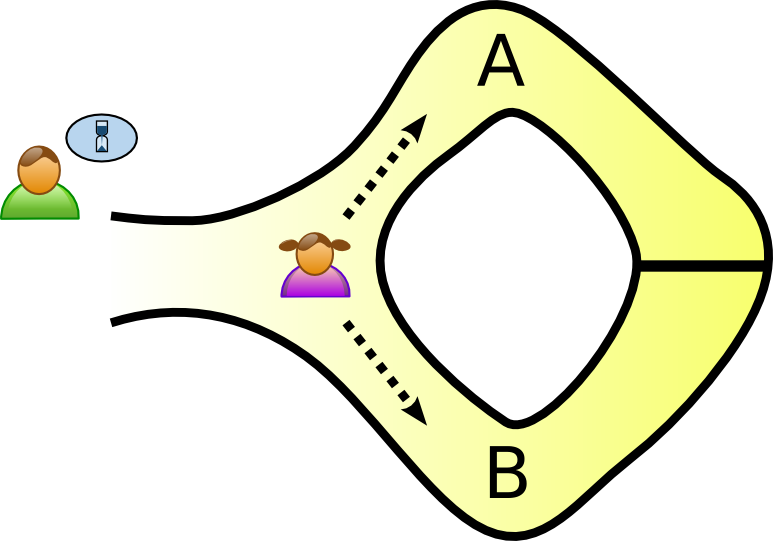
\includegraphics[height=2cm]{alibaba1.png} \\
        & \vspace{0cm}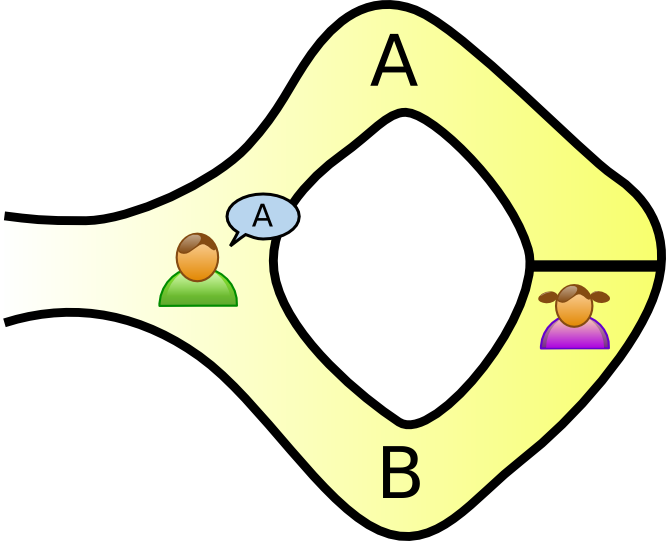
\includegraphics[height=2cm]{alibaba2.png} \\
        & \vspace{0cm}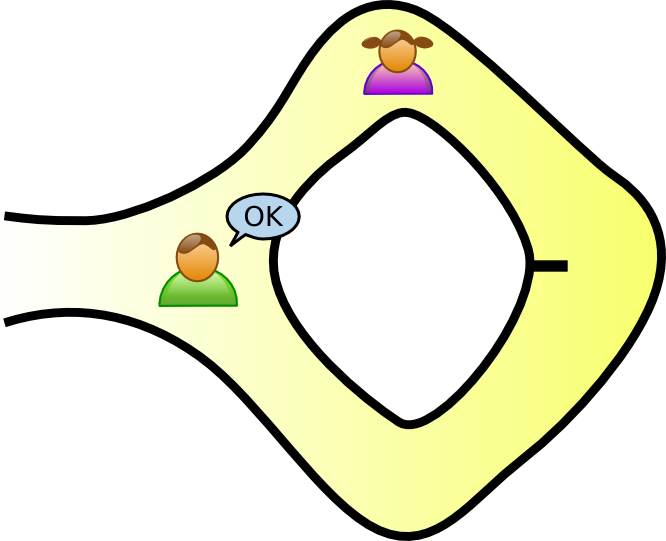
\includegraphics[height=2cm]{alibaba3.png} \\
    \end{tabular}
    
\end{frame}

\begin{frame}
    \frametitle{Camino Hamiltoniano}
    \begin{enumerate}
        \item{Peggy conoce un camino \~n Hamiltoniano de un grafo $\mathcal{G}$}
        \item{Peggy se lo quiere demostrar a Victor sin revelar el camino.}
        \item{Peggy crea un grafo $\mathcal{H}$, que es isomorfico a $\mathcal{G}$,
        en otras palabras, para cada vertice $g\in\mathcal{G}$ se define una biyeccion
        a los vertices $h\in\mathcal{H}$. Peggy no revela este isomorfismo.}
        \item{Peggy se compromete a dicho isomorfismo, posiblemente escribiendolo en
        un papel de tal manera que ella no lo puede cambiar.}
        \item{Victor debe escoger entre ver el isomorfismo o ver el camino Hamiltoniano:
            \begin{itemize}
                \item{Si Victor desea ver el isomorfismo, Peggy lo revela}
                \item{Si Victor desea ver el camino Hamiltoniano, Peggy revela
                dicho camino en el grafo $\mathcal{H}$ y solamente las esquinas
                utilizadas en el camino Hamiltoniano.}
            \end{itemize}
        }
    \end{enumerate}
\end{frame}

\begin{frame}
    \frametitle{Camino Hamiltoniano}
    \begin{tabular}{p{5cm} p{5cm}}
        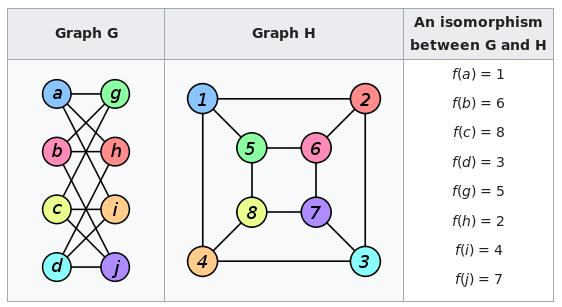
\includegraphics[width=5cm]{iso.png}
        & 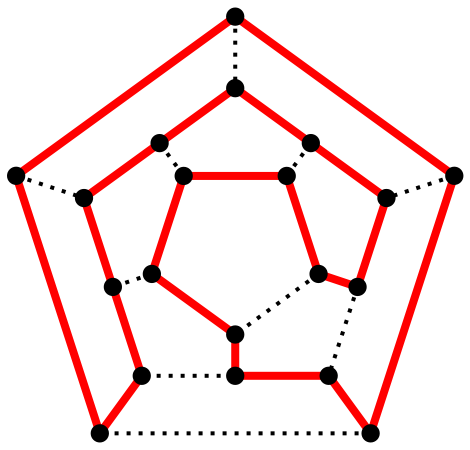
\includegraphics[width=5cm]{ham.png}
    \end{tabular}
\end{frame}

\begin{frame}
    \frametitle{Hashes}
    \begin{itemize}
        \item{Son un mapeo de objetos de un conjunto $\mathpzc{U}$
        a un conjunto m\'as peque\~no $\mathpzc{M}_{k}:=\{0,1,\dots,k\}$}
        \item{El conjunto $\mathpzc{U}$ puede ser cualquier colecci\'on de
        objetos: strings, matrices, personas, ect.}
        \item{Debido a que el conjunto $\mathpzc{U}$ es m\'as grande que
        el conjunto $\mathpzc{M}_k$, necesariamente existen \emph{colisiones}}
        \item{Una \emph{buena funci\'on de hasheo} distribuye sus colisiones
        de forma uniforme.}
    \end{itemize}
\end{frame}

\begin{frame}
    \frametitle{Applicaciones de Hahses}
    \begin{itemize}
        \item{Diccionarios}
        \item{Almacenamiento seguro de contrase\~nas}
        \item{Validaci\'on de integridad}
        \item{Proof of work}
    \end{itemize}
\end{frame}

\begin{frame}
    \frametitle{Hashes criptograficos y no-criptograficos}
    Un hash criptografico es dificil de invertir!
    \begin{itemize}
        \item{Los hashes no criptograficos solo evitan colisiones}
        \item{Dado un hash criptografico y un valor $m\in\mathpzc{M}_k$,
        es dificil obtener el valor original $u\in\mathpzc{U}$ que produjo
        dicho $m$. Idealmente, es tan dificil como una busqueda lineal.}
        \item{Un hash criptografico se debe comportar como una \emph{asignaci\'on aleatorea}
        en lo m\'as possible.}
        \item{Los hashes no-criptograficos son m\'as eficientes.}
    \end{itemize}
\end{frame}

\begin{frame}
    \frametitle{Ejemplos de Hashes criptograficos}
    \begin{itemize}
        \item{MD5: uno de los primeros, ahora no se considera seguro}
        \item{SHA-256: El hash criptografico m\'as usado. Se utiliza en
        el Blockchain de Bitcoin}
        \item{Scrybd: Intenta ser el m\'as caro de invertir. Aprovechando
        el costo de memoria ram. Se utiliza con los Litecoins.}
    \end{itemize}
{\bf Nota:} La distinci\'on entre hash criptografico y no criptografico
depende de la \emph{intenci\'on} de dicho hash. No su rendimiento.
\end{frame}

\end{document}